\documentclass[tikz]{standalone}
\usepackage{pgfplots}
\pgfplotsset{compat=1.15}
\usepackage{mathrsfs}
\usetikzlibrary{arrows,calc}
\usepackage{tkz-euclide}

\pagestyle{empty}

\definecolor{AngleClr}{rgb}{0,0.39215686274509803,0}
\definecolor{ShapeClr}{rgb}{0.6,0.2,0}

\begin{document}

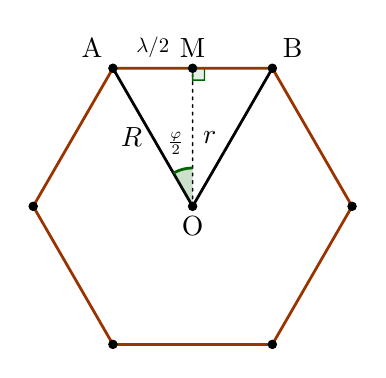
\begin{tikzpicture}[scale=.75]
\tkzSetUpLine[line width=1pt,color=black]
\tkzSetUpPoint[fill=black]

\tkzDefPoints{0/0/P0,2.7/0/P1}


\tkzDefRegPolygon[side,sides=6](P0,P1)

\tkzDefMidPoint(P4,P5) \tkzGetPoint{M}
\tkzDefCircle[circum](P1,P2,P3) \tkzGetPoint{O}


\tkzFillPolygon[fill=white](P1,P2,P3,P4,P5,P6)

\tkzDrawSegments[line width=0.5pt,color=black,dashed,dash pattern=on 1pt off 1.75pt](O,M)
\tkzDrawSegments[line width=1pt](O,P4 O,P5)

\tkzMarkRightAngles[line width=0.5pt, size=.2,color=AngleClr,fill=AngleClr,fill opacity=0.1](O,M,P4)

\tkzFillAngles[fill=AngleClr,size=.65,fill opacity=0.2](M,O,P5)
\tkzMarkAngles[line width=1pt,size=.65,color=AngleClr](M,O,P5)



\tkzDrawPolygon[color=ShapeClr](P1,P2,P3,P4,P5,P6)
\tkzDrawPoints[size=3](P1,P2,P3,P4,P5,P6,O,M)

\tkzLabelPoint[above right](P4){$\rm B$}
\tkzLabelPoint[above left](P5){$\rm A$}
\tkzLabelPoint[below](O){$\rm O$}
\tkzLabelPoint[above](M){$\rm M$}
\tkzLabelSegment[right](O,M){$r$}
\tkzLabelSegment[above](P5,M){\scalebox{0.75}{$\lambda/2$}}
\tkzLabelSegment[left](O,P5){$R$}

\tkzLabelAngle[pos=1.1](M,O,P5){\scalebox{0.75}{$\frac{\varphi}{2}$}}

\end{tikzpicture}

\end{document}
